\documentclass{homework}
\usepackage{homework}
\title{Week 2}
\date{}
\begin{document}
\maketitle
\section{Runge现象及等距节点插值和Chebyshev多项式插值逼近差异(P41/6)}
对$f(x)=\frac{1}{1+25x^2}$在$[0,1]$区间内进行等距节点的4、8、12阶多项式插值,和Chebyshev极值点的12阶多项式插值,并对比原函数图像。代码如下:
\lstinputlisting[language=Matlab]{Runge.m}
得到的图像如下:
\begin{figure}[H]
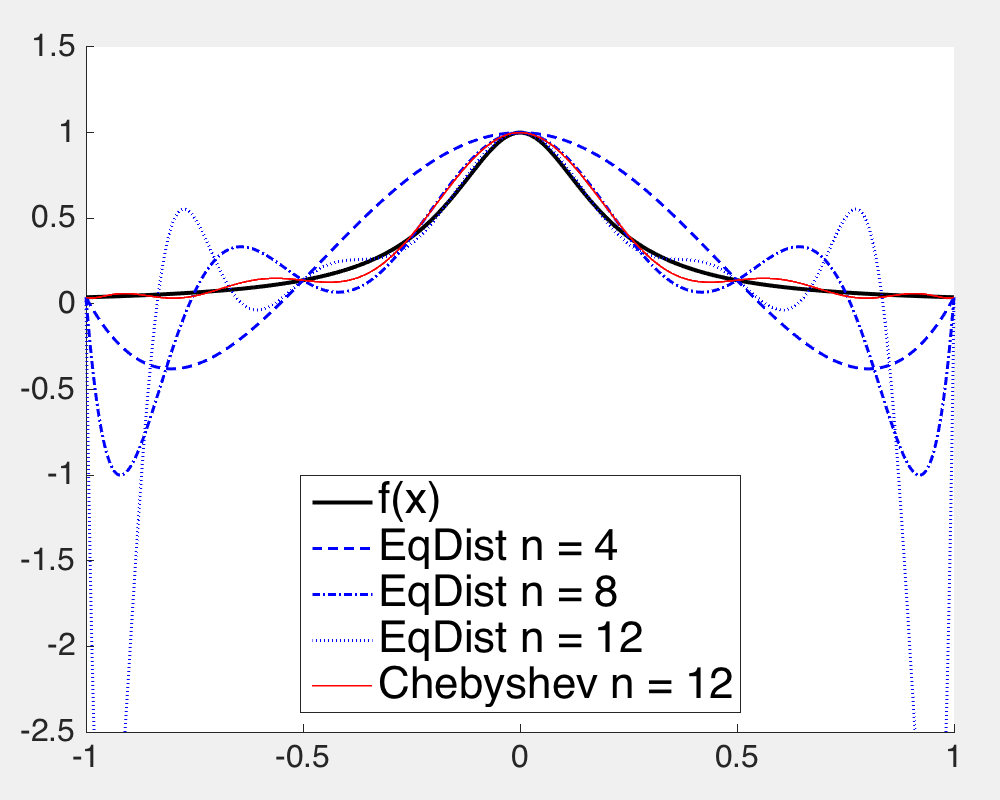
\includegraphics[width=9cm]{Runge.png}
\centering
\end{figure}
可以看到,随着节点书的增多,等距节点插值越来越不准确(Runge现象),当n=12时等距节点的插值在区间的两端已经出现了非常大的误差;而相对来说同阶的Chebyshev多项式插值则仍然有较好的逼近(但也难逃Runge现象),出现这样的差异主要因为Chebyshev极值点在区间两端附近节点密度增长的速率$\mathcal{O}(n^2)$比等距节点的速度$\mathcal{O}(n)$要快。
\section{用Newton公式计算$x^n$的积分(P43/表1.4)}
对$f(x)=x^n (n=1,2,3,4,5,6,7)$在$[0,1]$区间上进行Newton法数值积分。代码如下:
\lstinputlisting[language=Matlab]{NewtonInt.m}
得到的数据如下:
\begin{table}[H]
\caption{用Newton公式计算$x^n$的积分}
\centering
\begin{tabular}{|c|c|c|c|c|c|c|}
\hline
$x^n$ & 精确值 & 中点公式 & 梯形公式 & Simpson公式 & $\frac{3}{8}$规则 & Cotes公式 \\\hline
$x^1$ & 0.5000 & {\bf 0.5000} & {\bf 0.5000} & 0.5000 & 0.5000 & 0.5000 \\\hline
$x^2$ & 0.3333 & 0.2500 & 0.5000 & {\bf 0.3333} & 0.3333 & 0.3333 \\\hline
$x^3$ & 0.2500 & 0.1250 & 0.5000 & {\bf 0.2500} & {\bf 0.2500} & 0.2500 \\\hline
$x^4$ & 0.2000 & 0.0625 & 0.5000 & 0.2083 & 0.2037 & {\bf 0.2000} \\\hline
$x^5$ & 0.1667 & 0.0312 & 0.5000 & 0.1875 & 0.1759 & {\bf 0.1667} \\\hline
$x^6$ & 0.1429 & 0.0156 & 0.5000 & 0.1771 & 0.1584 & 0.1432 \\\hline
$x^7$ & 0.1250 & 0.0078 & 0.5000 & 0.1719 & 0.1471 & 0.1263 \\\hline
\end{tabular}
\end{table}
表中用粗体标出的数据和精确值吻合,由此可以看出来偶数n阶的数值积分公式对n+1次多项式也精确成立。
\section{用Gauss求积公式计算$x^n$的积分(P49/表1.5)}
由书48页公式可计算出n+1点的Gauss求积公式的节点和相对应权重:
\lstinputlisting[language=Matlab]{LegendreGauss.m}
上式求积区间为$[0,1]$,进行线性变换后便得到任意区间$[a,b]$上的Gauss求积公式:
\lstinputlisting[language=Matlab]{GaussInt.m}
由此便可以计算出$x^n$的k点Gauss求积结果:
\lstinputlisting[language=Matlab]{prob3.m}
得到的数据如下:
\begin{table}[H]
\centering
\caption{用Gauss公式计算$x^n$的积分}
\begin{tabular}{|c|c|c|c|c|c|c|}
\hline
$x^n$ & 精确值 & 1点 & 2点 & 3点 & 4点 & 5点 \\\hline
$x^1$ & 0.5000 & {\bf 0.5000} & 0.5000 & 0.5000 & 0.5000 & 0.5000 \\\hline
$x^2$ & 0.3333 & 0.2500 & {\bf 0.3333} & 0.3333 & 0.3333 & 0.3333 \\\hline
$x^3$ & 0.2500 & 0.1250 & {\bf 0.2500} & 0.2500 & 0.2500 & 0.2500 \\\hline
$x^4$ & 0.2000 & 0.0625 & 0.1944 & {\bf 0.2000} & 0.2000 & 0.2000 \\\hline
$x^5$ & 0.1667 & 0.0312 & 0.1528 & {\bf 0.1667} & 0.1667 & 0.1667 \\\hline
$x^6$ & 0.1429 & 0.0156 & 0.1204 & 0.1425 & {\bf 0.1429} & 0.1429 \\\hline
$x^7$ & 0.1250 & 0.0078 & 0.0949 & 0.1238 & {\bf 0.1250} & 0.1250 \\\hline
\end{tabular}
\end{table}
由加粗的精确值可以印证,n点的Gauss求积公式具有2n-1阶的代数精度。
\end{document}
